% Created 2012-10-14 Sun 17:53
\documentclass{article}
\usepackage[utf8]{inputenc}
\usepackage[T1]{fontenc}
\usepackage{fixltx2e}
\usepackage{graphicx}
\usepackage{longtable}
\usepackage{float}
\usepackage{wrapfig}
\usepackage{soul}
\usepackage{textcomp}
\usepackage{marvosym}
\usepackage{wasysym}
\usepackage{latexsym}
\usepackage{amssymb}
\usepackage{hyperref}
\tolerance=1000
\usepackage{color}
\usepackage{minted}
\usepackage{mathrsfs}
\usepackage{graphicx}
\usepackage{booktabs}
\usepackage{dcolumn}
\usepackage{subfigure}
\usepackage[margin=1in]{geometry}
\RequirePackage{fancyvrb}
\DefineVerbatimEnvironment{verbatim}{Verbatim}{fontsize=\small,formatcom = {\color[rgb]{0.1,0.2,0.9}}}
\providecommand{\alert}[1]{\textbf{#1}}

\title{}
\author{}
\date{\today}
\hypersetup{
  pdfkeywords={},
  pdfsubject={},
  pdfcreator={Emacs Org-mode version 7.8.02}}

\begin{document}



\setlength{\parindent}{0in}

\textbf{Interpretation of Coefficients and summary statistics in R} \hfill
\textbf{ARE213}: Section 01 \\ \\

The purpose of this section is twofold: (1) Basic review of the
interpretation of coefficients on common, linear models that we will
encounter in class. (2) Introduction and quick review of useful \texttt{R}
code to help with problem sets.  The section notes are an open-source,
Github project, which can be found here.  The text is an \texttt{org-mode}
document, which can be compiled as HTML or \LaTeX.  The text is
interactive, if you are an Emacs user: you can run the \texttt{R} code from
within the document, and then compile the results immediately.  If you
are interested in contributing to this project, see the readme on the
code repository, found here: \\

\href{https://github.com/danhammer/applied-metrics}{\texttt{https://github.com/danhammer/applied-metrics}}

\section*{Interpretation of Coefficients}
\label{sec-1}


The interpretation of the coefficients in a linear model depends on
the functional form of the covariates.  A common specification
involves the logarithms of the dependent and independent variables.
We will review each of the four cases below.  Note that a percentage
change in a variable $z$ is defined as $\% \Delta z =(100\cdot d
z)/{z}$.

\begin{enumerate}
\item \textbf{Linear-linear}: $y_i = \beta_0 + \beta_1 x_i + \epsilon_i$.  Then $d y_i =
   \beta_1 d x_i$ and $\beta_1 = d y_i / d x_i$.  A one unit change in
   $x_i$ will induce a one unit change in $y_i$.
\item \textbf{Log-linear}: $\log y_i = \beta_0 + \beta_1 x_i + \epsilon_i$. Then
   $d \log y_i = \beta_1 d x_i$.  Note that for small changes in
   $y_i$, $d \log y_i \approx (1/ y_i) d y_i$, such that $(1/ y_i) d
   y_i \approx \beta_1 d x_i$ and $[1/ (100 \cdot y_i)] d y_i \approx
   100 \cdot \beta_1 d x_i$.  A one unit change in $x_i$ generates a
   $\beta_1 \times 100$ percentage increase in $y_i$.  This model form
   is often used to estimate the impact of the returns to education: a
   one year increase in education leads to a $\beta_1 \times 100$ percent
   increase in wages.
\item \textbf{Linear-log}: $y_i = \beta_0 + \beta_1 \log x_i + \epsilon_i$. Then
   $d y_i = \beta_1 d \log x_i$.  Just as in the log-linear case, for
   small changes in $x_i$, $d \log x_i \approx (1/ x_i) d x_i$.  Thus,
   $d y_i \approx \beta_1 (d x_i / x_i)$, which implies that a 1\%
   change in $x_i$ results in a $\beta_1 / 100$ unit change in $y_i$.
\item \textbf{Log-log}: $\log y_i = \beta_0 + \beta_1 \log x_i + \epsilon_i$,
   such that $d \log y_i = \beta_1 d \log x_i$.  Using the results
   from the previous model specifications, it follows that $\beta_1 =
   (d y_i / y_i)/(d x_i / x_i)$.  The interpretation of $beta_1$ is
   the elasticity of $y_i$ with respect to $x_i$.  A one percentage
   change in $x_i$ will, on average, yield a $\beta_1$ percentage
   change in $y_i$.
\end{enumerate}
\section*{Tables and figures in R}
\label{sec-2}


If you are not familiar with \texttt{R}, then it might be useful to review
the section notes for ARE212, which can be found here: \\

\href{https://github.com/danhammer/ARE212}{\texttt{https://github.com/danhammer/ARE212}} \\

The ARE212 project gives a more rigorous introduction to econometrics
in \texttt{R}.  Here, we will review some basic commands to output
\LaTeX-ready tables and figures.  First, we will read in the data,
which has been saved as a \texttt{.dta} Stata file.  We will need to import
the \texttt{foreign} package to directly read the data set, without re-saving
it to a more common format.


\begin{minted}[]{r}
library(foreign)
data <- read.csv("../../../resources/ps1.csv")
\end{minted}

Ulitmately, we will try to estimate the impact of maternal smoking on
infant birthweight.  We can pare down the rather large data set into
one that represents only necessary variables for this impact analysis;
specifially, we will look at the infant birthweight (\texttt{dbrwt}),
maternal age (\texttt{dmage}), maternal education(\texttt{dmeduc}), paternal
eduaction (\texttt{dfeduc}), maternal cigarette usage (\texttt{cigar}), and marital
status of mother (\texttt{dmar}).  We will create a binary variable \texttt{smoker}
to indicate whether the mother used any cigarettes during pregnancy,
and we will drop observations with missing values for cigarette use:


\begin{minted}[]{r}
var.names <- c("dbrwt", "dmage", "dmeduc", "dmar", "dfeduc", "cigar")
good.vals <- data$cigar != 99
sm.data <- data[good.vals, var.names]
sm.data$smoker <- ifelse(sm.data$cigar > 0, 1, 0)
nrow(sm.data)
mean(sm.data$smoker)
\end{minted}

\begin{verbatim}
 [1] 119384
 [1] 0.165399
\end{verbatim}

Of the 119,384 observations in the sample, approximately 16.5\% were
associated with maternal smoking -- bad for the babies, but good for
variation of the \emph{treatment}.  We can run a few basic regressions,
appending the results into a single summary table, presented in Table
\ref{fig:regout}.


\begin{minted}[]{r}
library(texreg)
model1 <- lm(dbrwt ~ smoker, data=sm.data)
model2 <- lm(dbrwt ~ smoker + dmage + dmeduc, data=sm.data)
model3 <- lm(dbrwt ~ smoker + dmage + dmeduc + dmar + dfeduc, data=sm.data)
table.string <- texreg(list(model1, model2, model3), 
                       caption = "regression output",
                       float.pos = "b!",
                       label = "fig:regout",
                       use.packages = FALSE)
\end{minted}

 
\begin{table}[b!]
\begin{center}
\begin{tabular}{l D{.}{.}{6.5} @{}D{.}{.}{6.5} @{}D{.}{.}{6.5} @{}}
\toprule
            & \multicolumn{1}{c}{Model 1} & \multicolumn{1}{c}{Model 2} & \multicolumn{1}{c}{Model 3} \\
\midrule
(Intercept) & 3407.22^{***} & 3115.57^{***} & 3487.86^{***} \\
            & (1.85)        & (11.34)       & (16.52)       \\
smoker      & -250.50^{***} & -226.94^{***} & -197.37^{***} \\
            & (4.56)        & (4.68)        & (4.74)        \\
dmage       &               & 6.56^{***}    & 1.89^{***}    \\
            &               & (0.33)        & (0.35)        \\
dmeduc      &               & 8.02^{***}    & 2.35^{**}     \\
            &               & (0.84)        & (1.03)        \\
dmar        &               &               & -154.67^{***} \\
            &               &               & (4.54)        \\
dfeduc      &               &               & 1.64^{*}      \\
            &               &               & (0.98)        \\
\midrule
R$^2$       & 0.02          & 0.03          & 0.04          \\
Adj. R$^2$  & 0.02          & 0.03          & 0.04          \\
Num. obs.   & 119384        & 119384        & 119384        \\
\bottomrule
\vspace{-2mm}\\
\multicolumn{4}{l}{\textsuperscript{***}$p<0.01$, \textsuperscript{**}$p<0.05$, \textsuperscript{*}$p<0.1$}
\end{tabular}
\end{center}
\caption{regression output}
\label{fig:regout}
\end{table}

If you want to save the output as a \LaTeX fragment in order to use
the \texttt{\textbackslash{}input\{\}} command (e.g., \texttt{\textbackslash{}input\{regout.tex\}}) then you can add
the following lines to save it to the appropriate file.  Otherwise,
you can copy and paste the output of the \texttt{texreg} into your \texttt{.tex}
file.


\begin{minted}[]{r}
out <- capture.output(cat(table.string))
cat(out, file="regout.tex", sep="\n")
\end{minted}

Next, suppose we want to create a kernel density plot of infant
birthweight for smoking mothers and non-smoking mothers.  For this, we
will rely on the very powerful \texttt{ggplot2} package.  There are a lot of
online resources for \texttt{ggplot2}, including (shameless pitch) the code
found in the ARE212 repository.  We plot the kernel densities with the
\texttt{R} defaults, as well as the count histograms.


\begin{minted}[]{r}
library(ggplot2)
sm.data$condition <- ifelse(sm.data$smoker == 1, "smoker", "non-smoker")
ggplot(sm.data, aes(x=dbrwt, fill=condition)) + geom_density(alpha=0.2)
\end{minted}

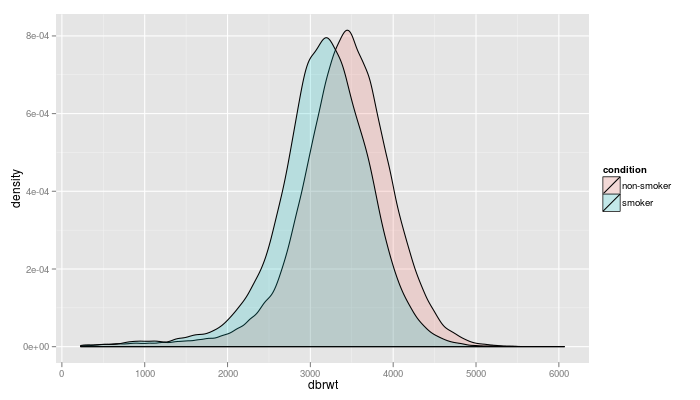
\includegraphics[width=.9\linewidth]{fig1.png}



\begin{minted}[]{r}
ggplot(sm.data, aes(x=dbrwt, fill=condition)) + geom_histogram(position="identity")
\end{minted}

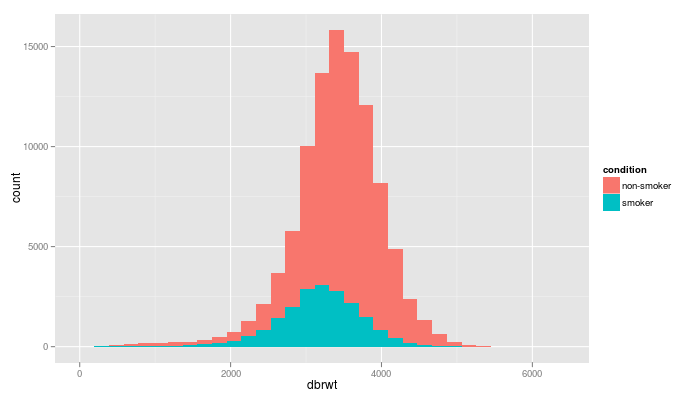
\includegraphics[width=.9\linewidth]{fig2.png}

\end{document}
